\begin{easyappendix}{Wizualizacje estymacji}

    \begin{table}[H]
        \centering
        \caption{Wizualizacje estymacji na obrazie z zestawu Taskonomy.}
        \vspace{0.1cm}
        \resizebox{\textwidth}{!}{%
            \begin{tabular}{ |m{3cm}|p{3cm}| }
            \hline
            Nazwa algorytmu & Wizualizacja \\
            \hline \hline
            AdelaiDepth &
            \begin{figure}[H]
                \centering
                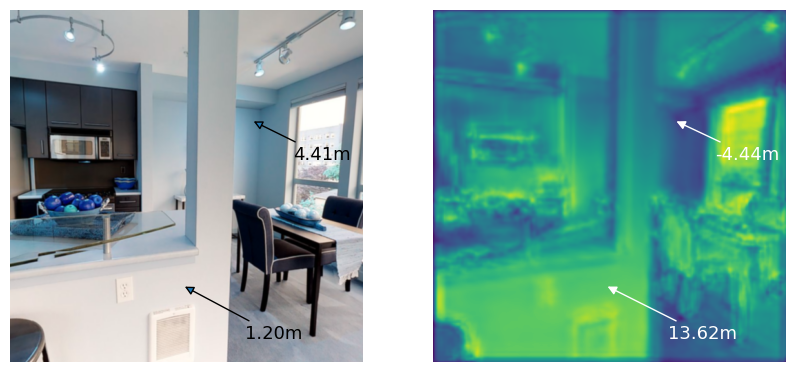
\includegraphics[width=1\textwidth]{comparison/adelai-tasko1.png}
            \end{figure} \\
            \hline
            MetaPrompt-SD &
            \begin{figure}[H]
                \centering
                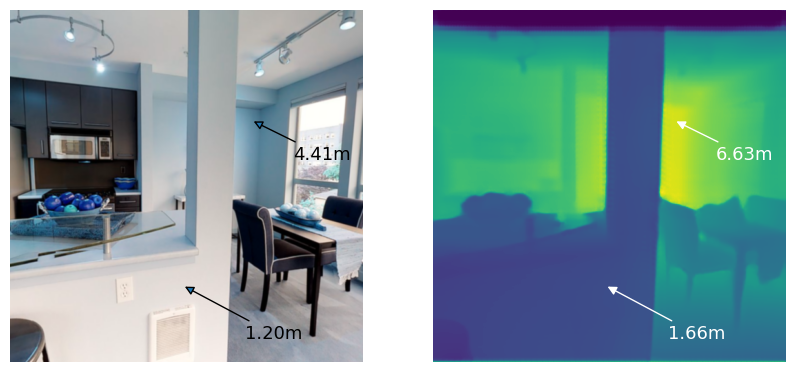
\includegraphics[width=1\textwidth]{comparison/meta-tasko1.png}
            \end{figure} \\
            \hline
            \end{tabular}%
        }
        \label{tab:vis-beg}
    \end{table}
    \begin{table}[H]
        \centering
        \vspace{0.1cm}
        \resizebox{\textwidth}{!}{%
            \begin{tabular}{ |m{3cm}|p{3cm}| }
            \hline
            DepthAnythingV2 &
            \begin{figure}[H]
                \centering
                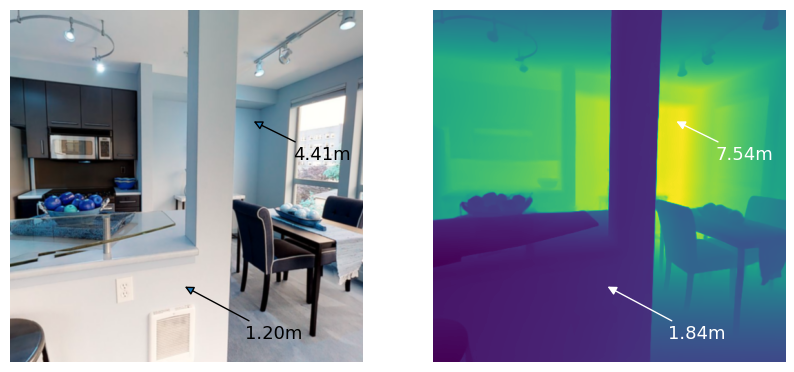
\includegraphics[width=1\textwidth]{comparison/depth-tasko1.png}
            \end{figure} \\
            \hline
            Metric3D &
            \begin{figure}[H]
                \centering
                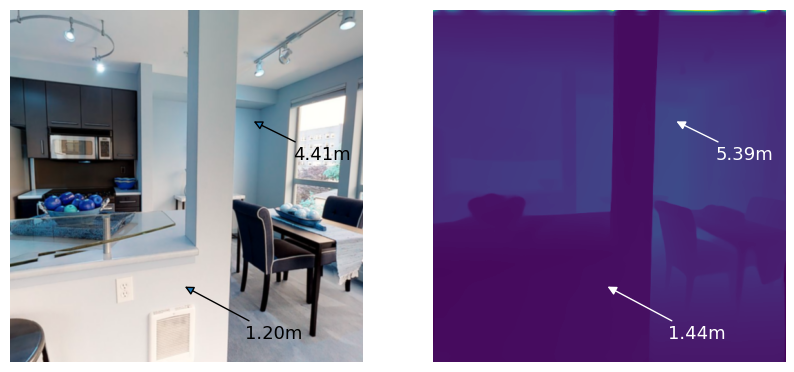
\includegraphics[width=1\textwidth]{comparison/metric-tasko1.png}
            \end{figure} \\
            \hline
            GCNDepth &
            \begin{figure}[H]
                \centering
                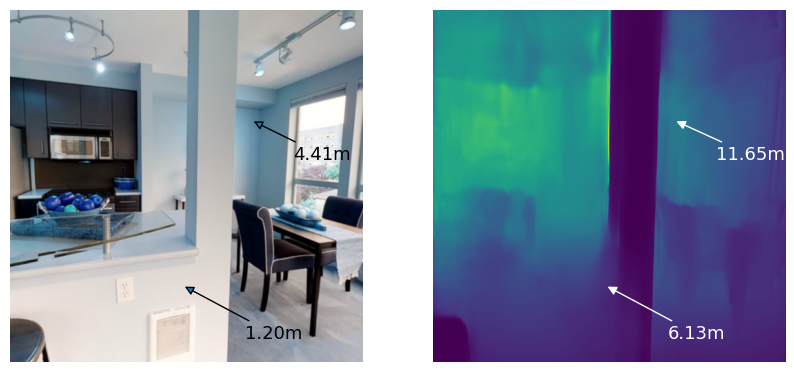
\includegraphics[width=1\textwidth]{comparison/gcn-tasko1.png}
            \end{figure} \\
            \hline
            \end{tabular}%
        }
    \end{table}
    \begin{table}[H]
        \centering
        \vspace{0.1cm}
        \resizebox{\textwidth}{!}{%
            \begin{tabular}{ |m{3cm}|p{3cm}| }
            \hline
            SQLdepth &
            \begin{figure}[H]
                \centering
                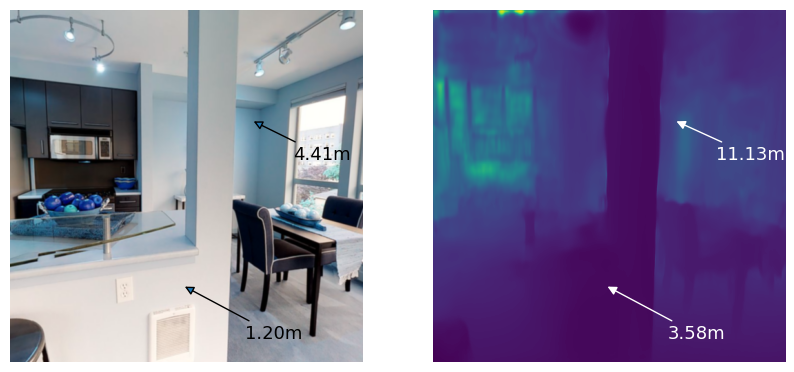
\includegraphics[width=1\textwidth]{comparison/sql-tasko1.png}
            \end{figure} \\
            \hline
            \end{tabular}%
        }
    \end{table}

    \begin{table}[H]
        \centering
        \caption{Wizualizacje estymacji na kolejnym obrazie z zestawu Taskonomy.}
        \vspace{0.1cm}
        \resizebox{\textwidth}{!}{%
            \begin{tabular}{ |m{3cm}|p{3cm}| }
            \hline
            Nazwa algorytmu & Wizualizacja \\
            \hline \hline
            AdelaiDepth &
            \begin{figure}[H]
                \centering
                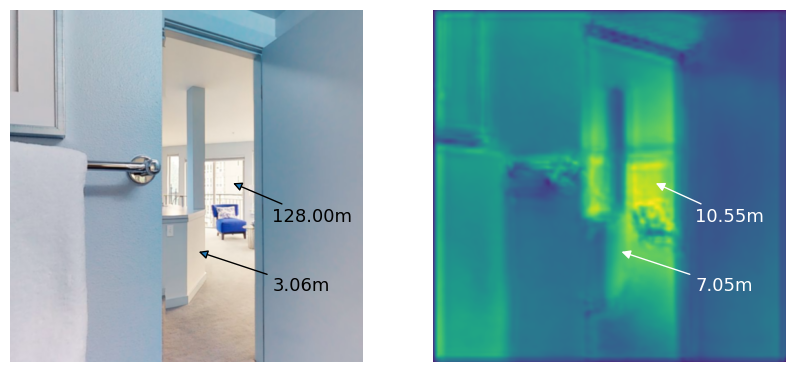
\includegraphics[width=1\textwidth]{comparison/adelai-tasko2.png}
            \end{figure} \\
            \hline
            \end{tabular}%
        }
    \end{table}
    \begin{table}[H]
        \centering
        \vspace{0.1cm}
        \resizebox{\textwidth}{!}{%
            \begin{tabular}{ |m{3cm}|p{3cm}| }
            \hline
            MetaPrompt-SD &
            \begin{figure}[H]
                \centering
                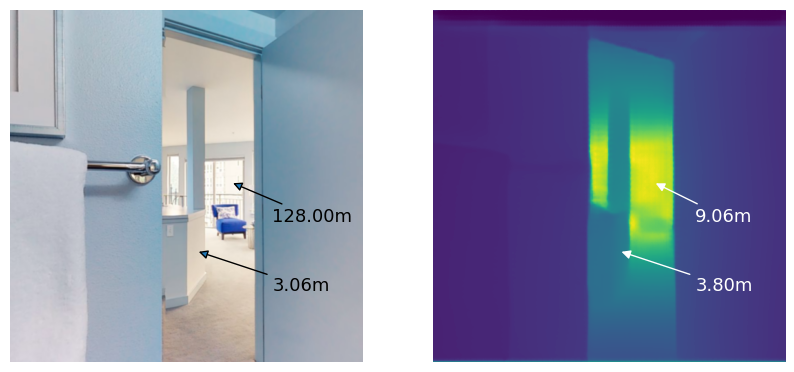
\includegraphics[width=1\textwidth]{comparison/meta-tasko2.png}
            \end{figure} \\
            \hline
            DepthAnythingV2 &
            \begin{figure}[H]
                \centering
                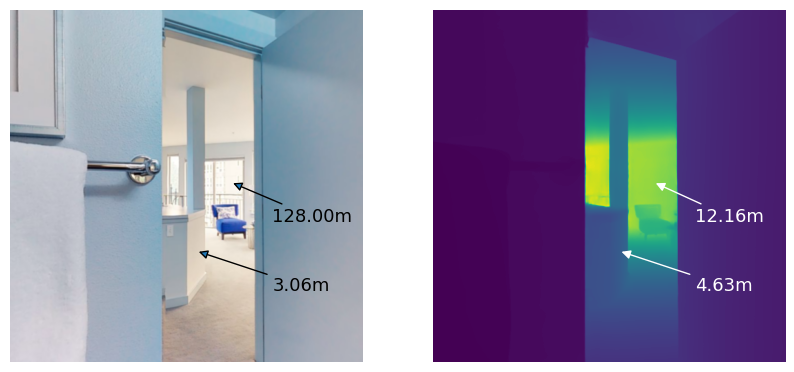
\includegraphics[width=1\textwidth]{comparison/depth-tasko2.png}
            \end{figure} \\
            \hline
            Metric3D &
            \begin{figure}[H]
                \centering
                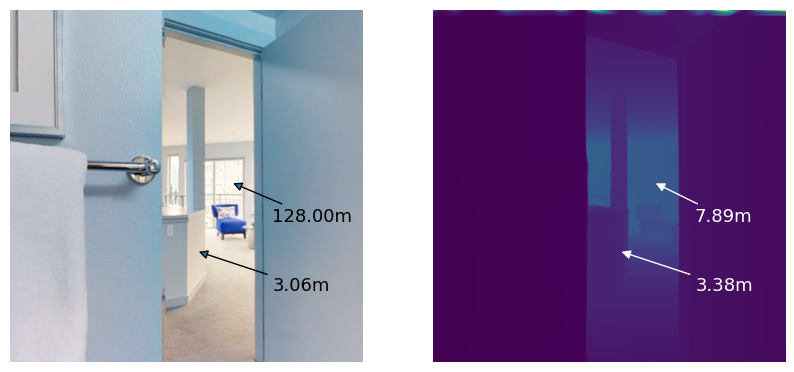
\includegraphics[width=1\textwidth]{comparison/metric-tasko2.png}
            \end{figure} \\
            \hline
            \end{tabular}%
        }
    \end{table}
    \begin{table}[H]
        \centering
        \vspace{0.1cm}
        \resizebox{\textwidth}{!}{%
            \begin{tabular}{ |m{3cm}|p{3cm}| }
            \hline
            GCNDepth &
            \begin{figure}[H]
                \centering
                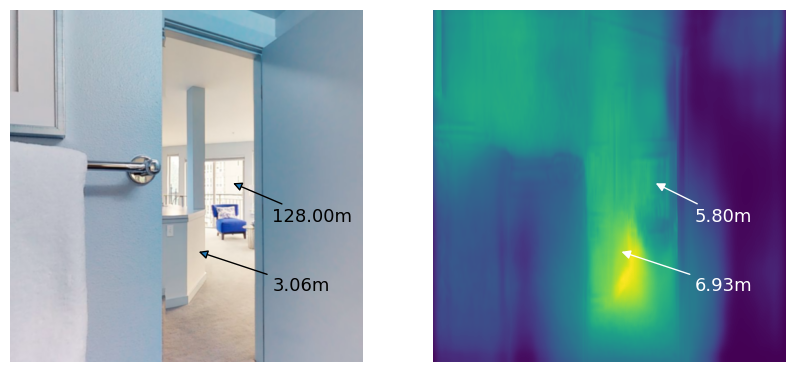
\includegraphics[width=1\textwidth]{comparison/gcn-tasko2.png}
            \end{figure} \\
            \hline
            SQLdepth &
            \begin{figure}[H]
                \centering
                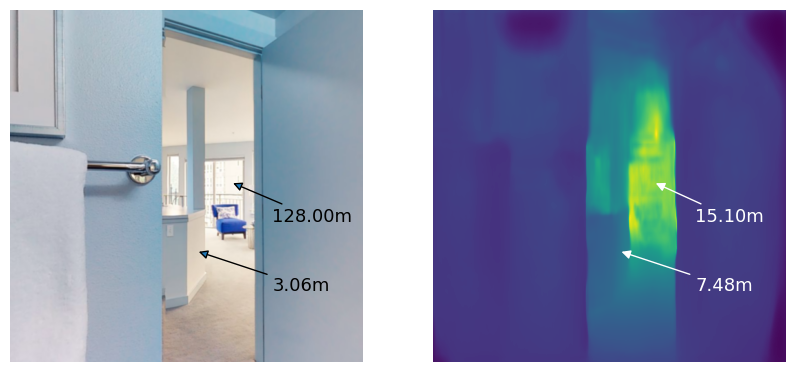
\includegraphics[width=1\textwidth]{comparison/sql-tasko2.png}
            \end{figure} \\
            \hline
            \end{tabular}%
        }
    \end{table}

    \begin{table}[H]
        \centering
        \caption{Wizualizacje estymacji na obrazie z zestawu austorskiego.}
        \vspace{0.1cm}
        \resizebox{\textwidth}{!}{%
            \begin{tabular}{ |m{3cm}|p{3cm}| }
            \hline
            Nazwa algorytmu & Wizualizacja \\
            \hline \hline
            AdelaiDepth &
            \begin{figure}[H]
                \centering
                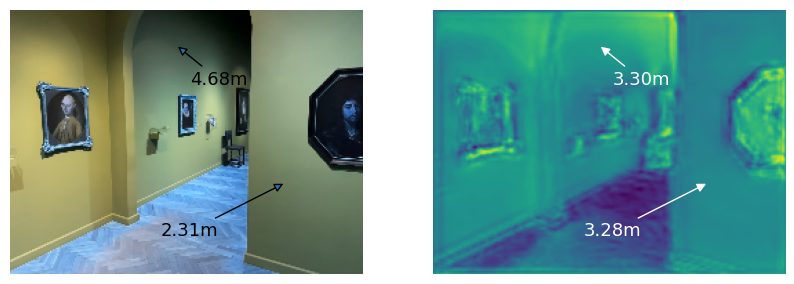
\includegraphics[width=1\textwidth]{comparison/adelai-stray1.png}
            \end{figure} \\
            \hline
            \end{tabular}%
        }
    \end{table}
    \begin{table}[H]
        \centering
        \vspace{0.1cm}
        \resizebox{\textwidth}{!}{%
            \begin{tabular}{ |m{3cm}|p{3cm}| }
            \hline
            MetaPrompt-SD &
            \begin{figure}[H]
                \centering
                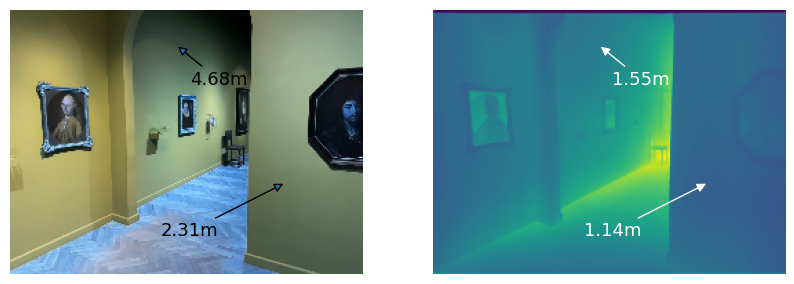
\includegraphics[width=1\textwidth]{comparison/meta-stray1.png}
            \end{figure} \\
            \hline
            DepthAnythingV2 &
            \begin{figure}[H]
                \centering
                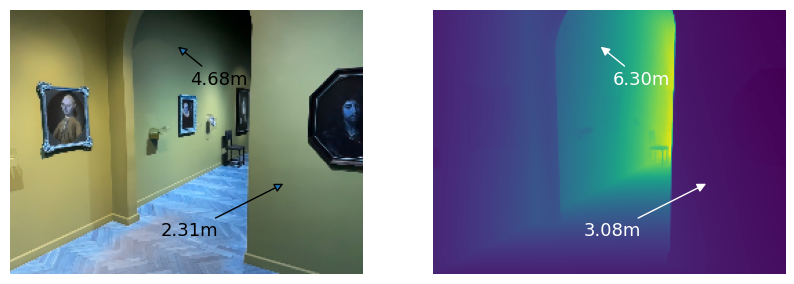
\includegraphics[width=1\textwidth]{comparison/depth-stray1.png}
            \end{figure} \\
            \hline
            Metric3D &
            \begin{figure}[H]
                \centering
                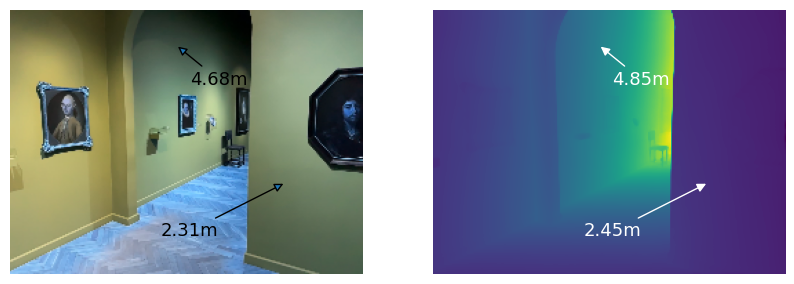
\includegraphics[width=1\textwidth]{comparison/metric-stray1.png}
            \end{figure} \\
            \hline
            \end{tabular}%
        }
    \end{table}
    \begin{table}[H]
        \centering
        \vspace{0.1cm}
        \resizebox{\textwidth}{!}{%
            \begin{tabular}{ |m{3cm}|p{3cm}| }
            \hline
            GCNDepth &
            \begin{figure}[H]
                \centering
                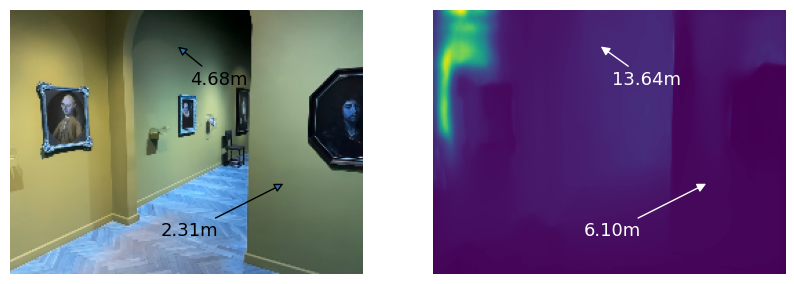
\includegraphics[width=1\textwidth]{comparison/gcn-stray1.png}
            \end{figure} \\
            \hline
            SQLdepth &
            \begin{figure}[H]
                \centering
                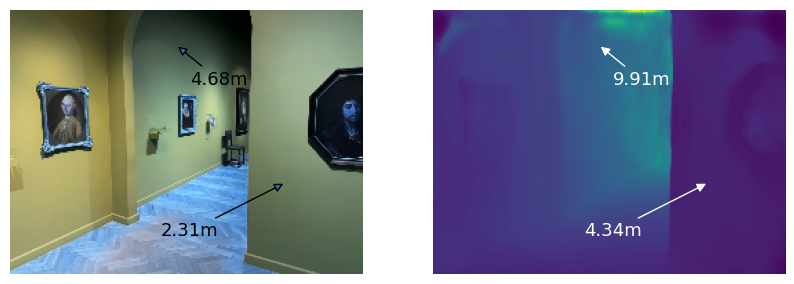
\includegraphics[width=1\textwidth]{comparison/sql-stray1.png}
            \end{figure} \\
            \hline
            \end{tabular}%
        }
    \end{table}

    \begin{table}[H]
        \centering
        \caption{Wizualizacje estymacji na kolejnym obrazie z zestawu austorskiego.}
        \vspace{0.1cm}
        \resizebox{\textwidth}{!}{%
            \begin{tabular}{ |m{3cm}|p{3cm}| }
            \hline
            Nazwa algorytmu & Wizualizacja \\
            \hline \hline
            AdelaiDepth &
            \begin{figure}[H]
                \centering
                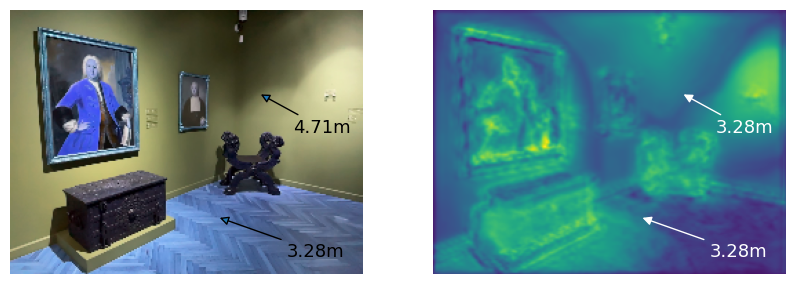
\includegraphics[width=1\textwidth]{comparison/adelai-stray2.png}
            \end{figure} \\
            \hline
            \end{tabular}%
        }
    \end{table}
    \begin{table}[H]
        \centering
        \vspace{0.1cm}
        \resizebox{\textwidth}{!}{%
            \begin{tabular}{ |m{3cm}|p{3cm}| }
            \hline
            MetaPrompt-SD &
            \begin{figure}[H]
                \centering
                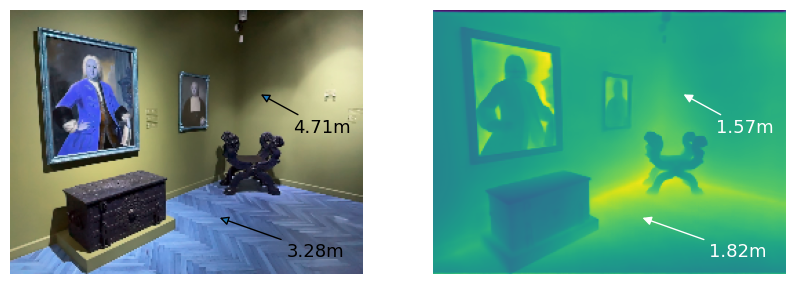
\includegraphics[width=1\textwidth]{comparison/meta-stray2.png}
            \end{figure} \\
            \hline
            DepthAnythingV2 &
            \begin{figure}[H]
                \centering
                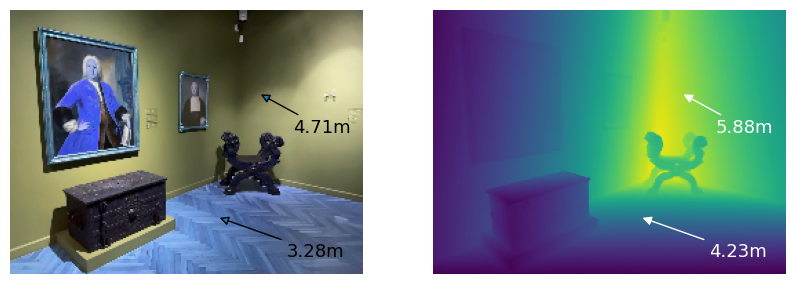
\includegraphics[width=1\textwidth]{comparison/depth-stray2.png}
            \end{figure} \\
            \hline
            Metric3D &
            \begin{figure}[H]
                \centering
                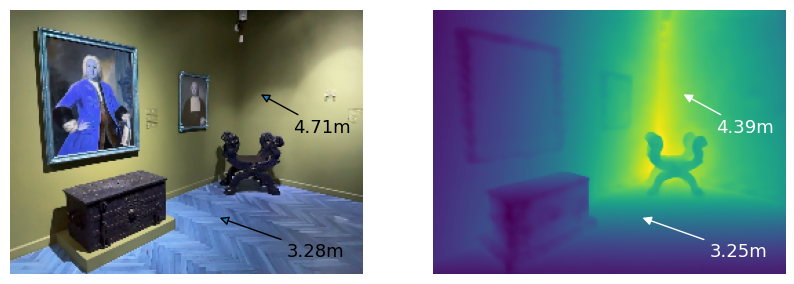
\includegraphics[width=1\textwidth]{comparison/metric-stray2.png}
            \end{figure} \\
            \hline
            \end{tabular}%
        }
    \end{table}
    \begin{table}[H]
        \centering
        \vspace{0.1cm}
        \resizebox{\textwidth}{!}{%
            \begin{tabular}{ |m{3cm}|p{3cm}| }
            \hline
            GCNDepth &
            \begin{figure}[H]
                \centering
                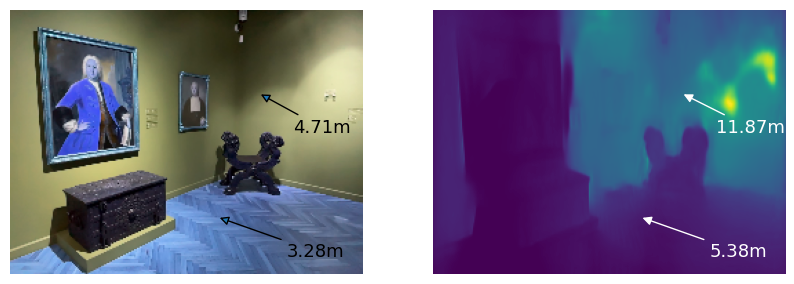
\includegraphics[width=1\textwidth]{comparison/gcn-stray2.png}
            \end{figure} \\
            \hline
            SQLdepth &
            \begin{figure}[H]
                \centering
                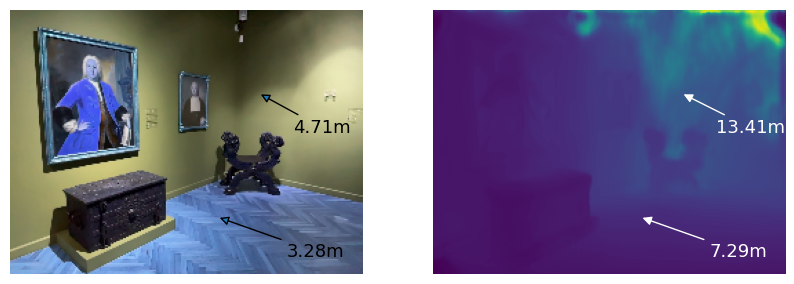
\includegraphics[width=1\textwidth]{comparison/sql-stray2.png}
            \end{figure} \\
            \hline
            \end{tabular}%
        }
    \end{table}

    \begin{table}[H]
        \centering
        \caption{Wizualizacje estymacji na obrazie z zestawu DIODE.}
        \vspace{0.1cm}
        \resizebox{\textwidth}{!}{%
            \begin{tabular}{ |m{3cm}|p{3cm}| }
            \hline
            Nazwa algorytmu & Wizualizacja \\
            \hline \hline
            AdelaiDepth &
            \begin{figure}[H]
                \centering
                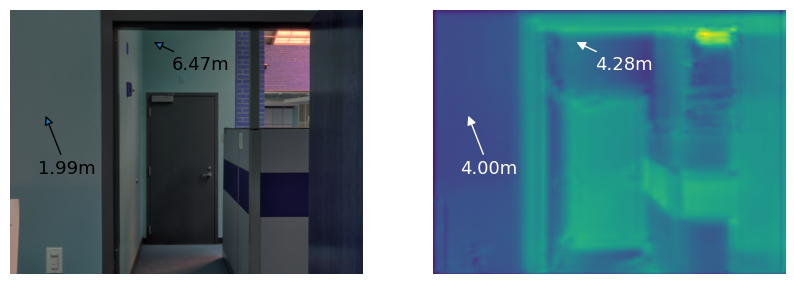
\includegraphics[width=1\textwidth]{comparison/adelai-diode.png}
            \end{figure} \\
            \hline
            \end{tabular}%
        }
    \end{table}
    \begin{table}[H]
        \centering
        \vspace{0.1cm}
        \resizebox{\textwidth}{!}{%
            \begin{tabular}{ |m{3cm}|p{3cm}| }
            \hline
            MetaPrompt-SD &
            \begin{figure}[H]
                \centering
                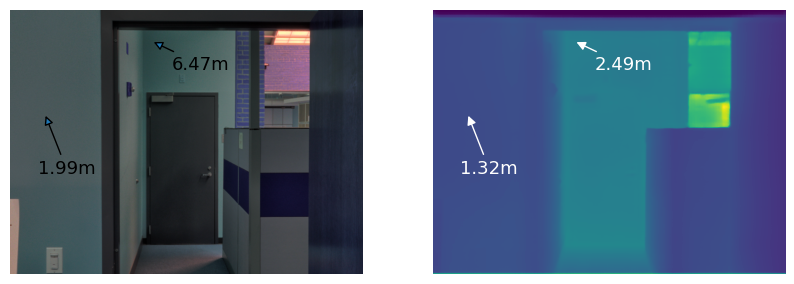
\includegraphics[width=1\textwidth]{comparison/meta-diode.png}
            \end{figure} \\
            \hline
            DepthAnythingV2 &
            \begin{figure}[H]
                \centering
                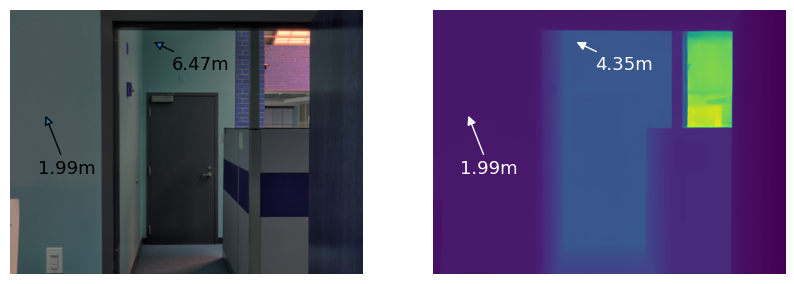
\includegraphics[width=1\textwidth]{comparison/depth-diode.png}
            \end{figure} \\
            \hline
            Metric3D &
            \begin{figure}[H]
                \centering
                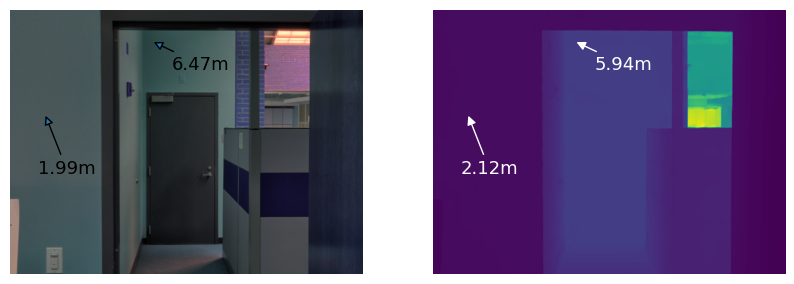
\includegraphics[width=1\textwidth]{comparison/metric-diode.png}
            \end{figure} \\
            \hline
            \end{tabular}%
        }
    \end{table}
    \begin{table}[H]
        \centering
        \vspace{0.1cm}
        \resizebox{\textwidth}{!}{%
            \begin{tabular}{ |m{3cm}|p{3cm}| }
            \hline
            GCNDepth &
            \begin{figure}[H]
                \centering
                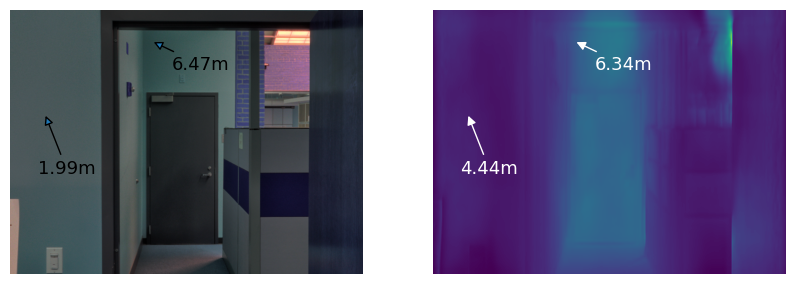
\includegraphics[width=1\textwidth]{comparison/gcn-diode.png}
            \end{figure} \\
            \hline
            SQLdepth &
            \begin{figure}[H]
                \centering
                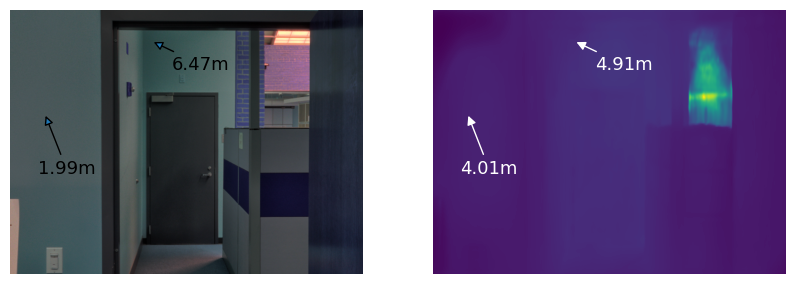
\includegraphics[width=1\textwidth]{comparison/sql-diode.png}
            \end{figure} \\
            \hline
            \end{tabular}%
        }
    \end{table}

    \begin{table}[H]
        \centering
        \caption{Wizualizacje estymacji na obrazie z zestawu KITTI.}
        \vspace{0.1cm}
        \resizebox{\textwidth}{!}{%
            \begin{tabular}{ |m{3cm}|p{3cm}| }
            \hline
            Nazwa algorytmu & Wizualizacja \\
            \hline \hline
            AdelaiDepth &
            \begin{figure}[H]
                \centering
                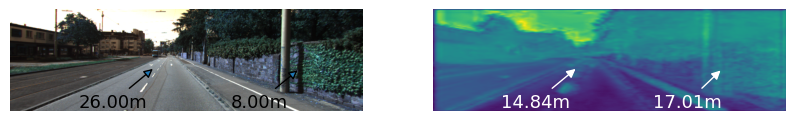
\includegraphics[width=1\textwidth]{comparison/adelai-kitti.png}
            \end{figure} \\
            \hline
            MetaPrompt-SD &
            \begin{figure}[H]
                \centering
                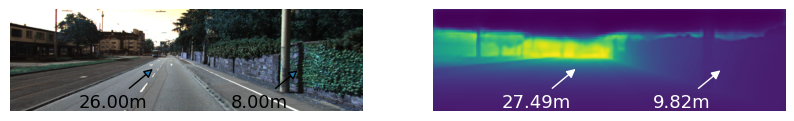
\includegraphics[width=1\textwidth]{comparison/meta-kitti.png}
            \end{figure} \\
            \hline
        \end{tabular}%
        }
        \label{tab:vis-end}
    \end{table}
    \begin{table}[H]
        \centering
        \vspace{0.1cm}
        \resizebox{\textwidth}{!}{%
            \begin{tabular}{ |m{3cm}|p{3cm}| }
            \hline
            DepthAnythingV2 &
            \begin{figure}[H]
                \centering
                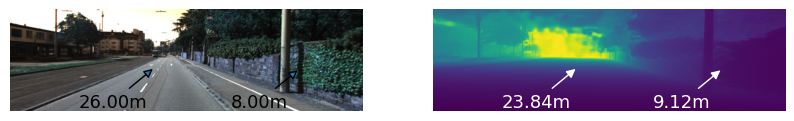
\includegraphics[width=1\textwidth]{comparison/depth-kitti.png}
            \end{figure} \\
            \hline
            Metric3D &
            \begin{figure}[H]
                \centering
                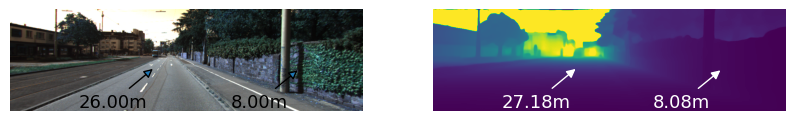
\includegraphics[width=1\textwidth]{comparison/metric-kitti.png}
            \end{figure} \\
            \hline
            GCNDepth &
            \begin{figure}[H]
                \centering
                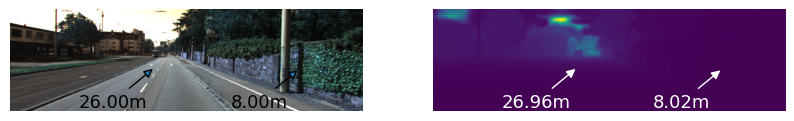
\includegraphics[width=1\textwidth]{comparison/gcn-kitti.png}
            \end{figure} \\
            \hline
            SQLdepth &
            \begin{figure}[H]
                \centering
                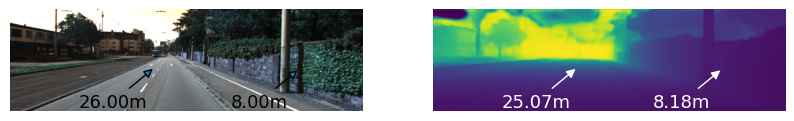
\includegraphics[width=1\textwidth]{comparison/sql-kitti.png}
            \end{figure} \\
            \hline
            \end{tabular}%
        }
    \end{table}

\end{easyappendix}

\begin{easyappendix}{Autorski zestaw danych}

    \begin{figure}[H]
        \centering
        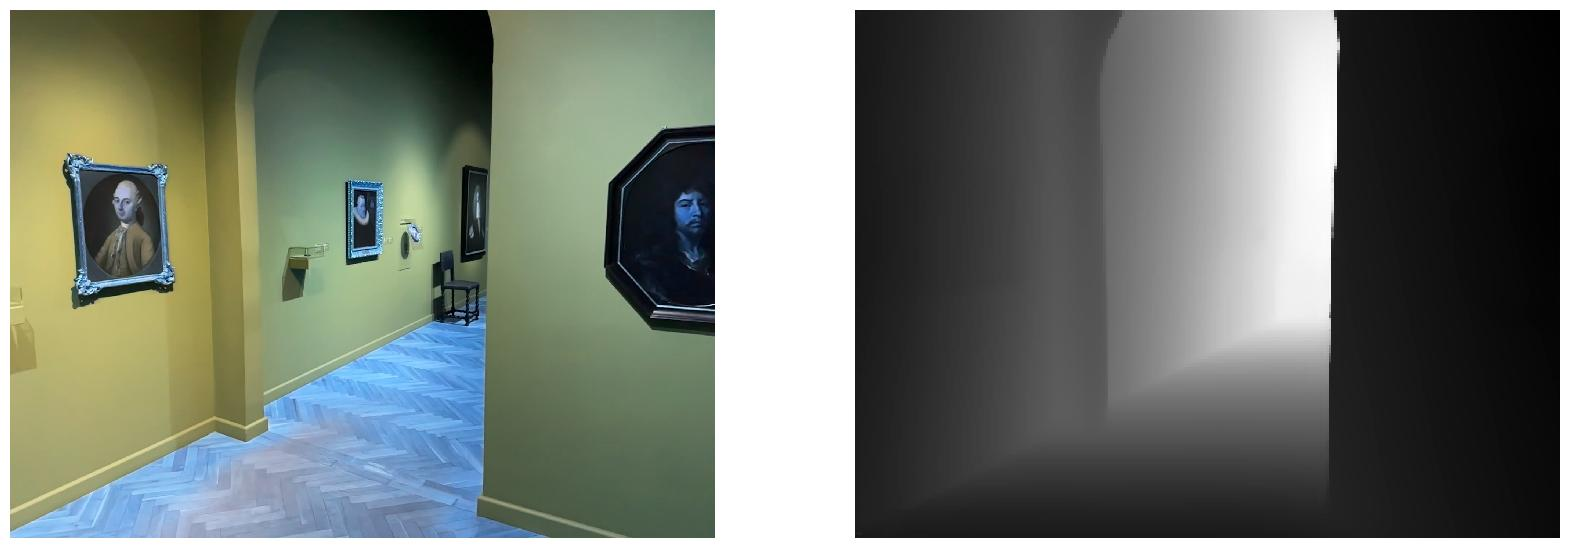
\includegraphics[width=0.9\textwidth]{dataset/plt_651f0aefef.jpg}
    \end{figure}
    \begin{figure}[H]
        \centering
        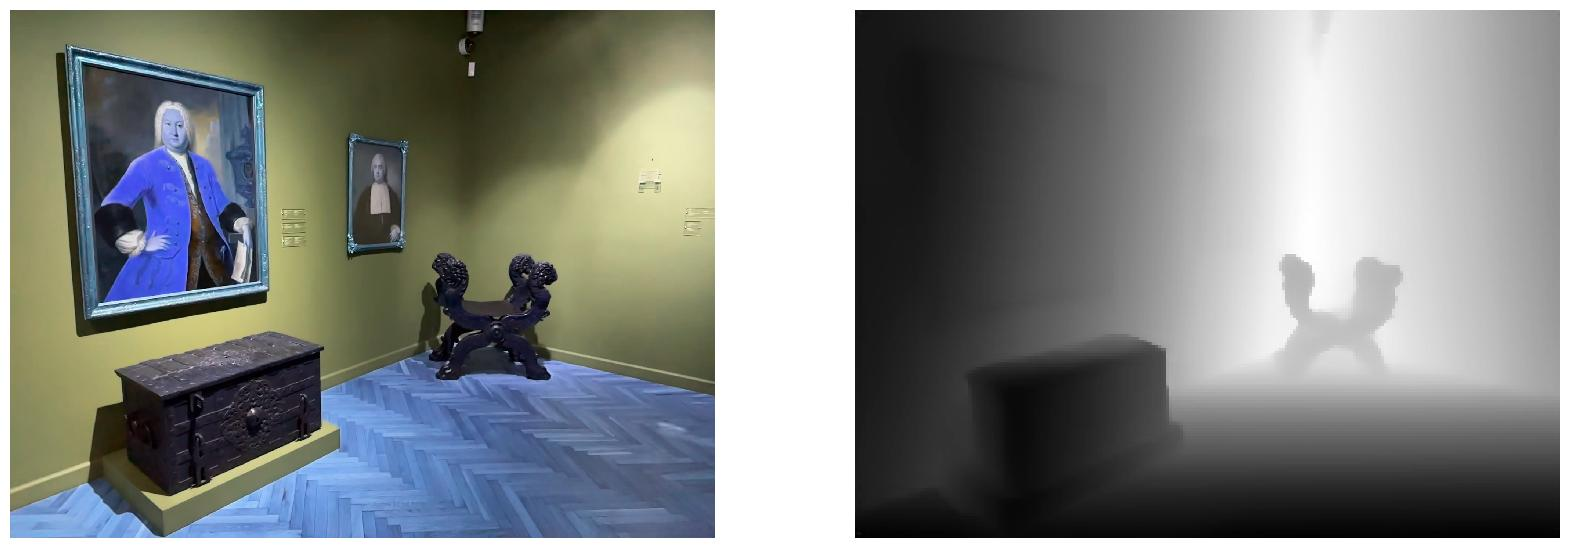
\includegraphics[width=0.9\textwidth]{dataset/plt_656af8e597.jpg}
    \end{figure}
    \begin{figure}[H]
        \centering
        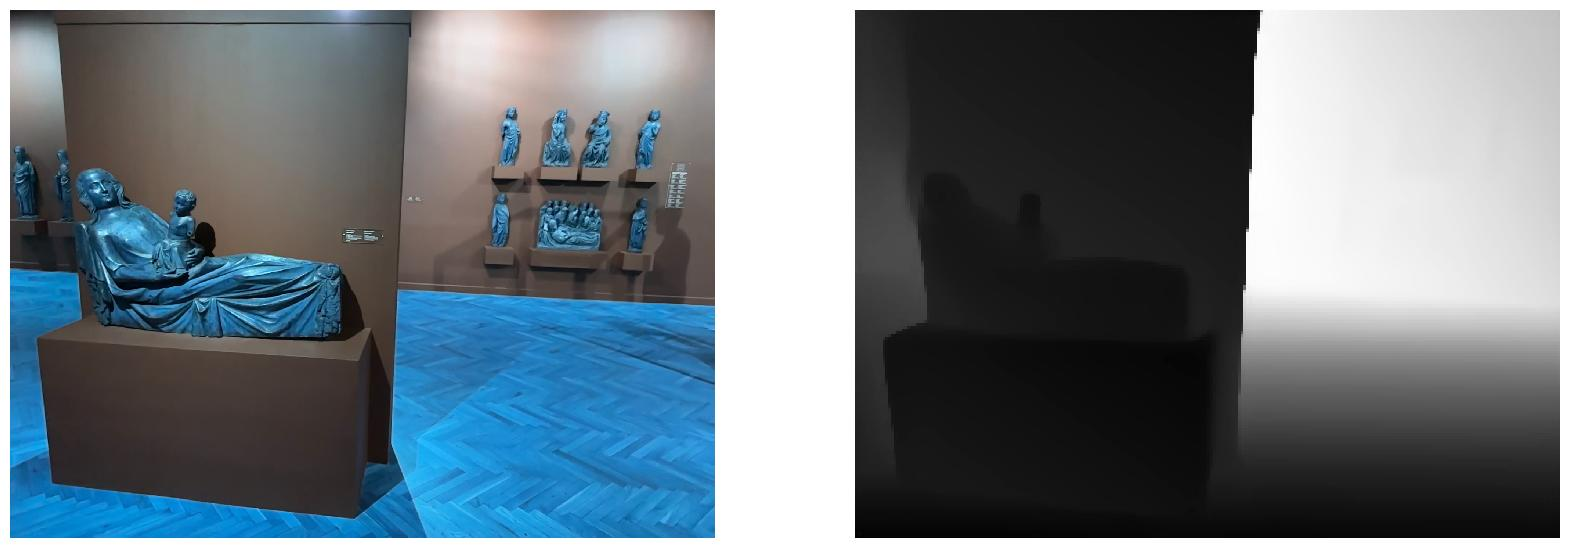
\includegraphics[width=0.9\textwidth]{dataset/plt_738eb8bcad.jpg}
    \end{figure}
    \begin{figure}[H]
        \centering
        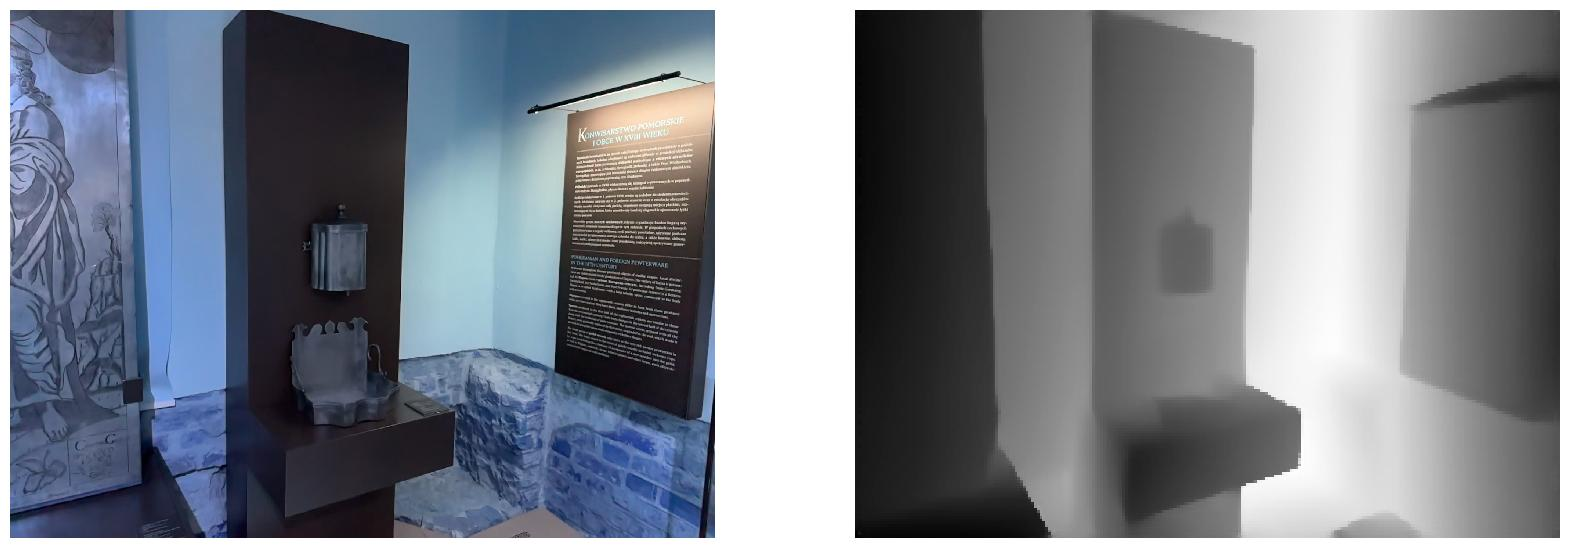
\includegraphics[width=0.9\textwidth]{dataset/plt_876ceff8d9.jpg}
    \end{figure}
    \begin{figure}[H]
        \centering
        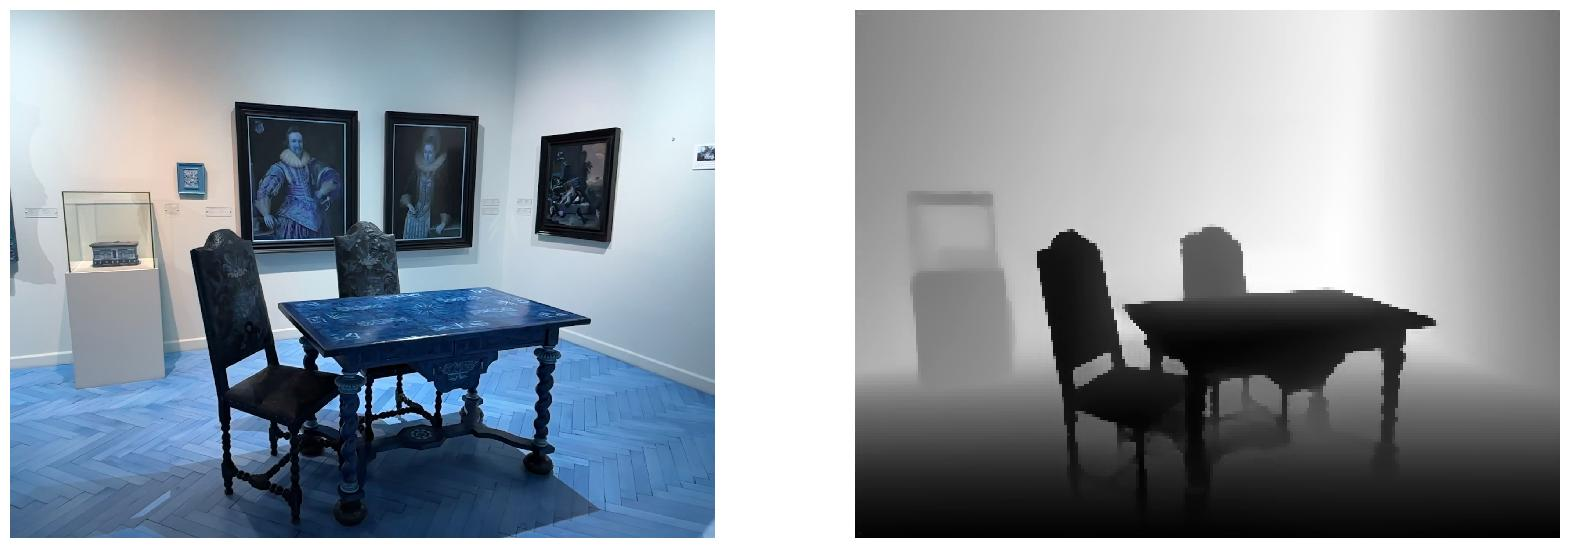
\includegraphics[width=0.9\textwidth]{dataset/plt_8276604808.jpg}
    \end{figure}
    \begin{figure}[H]
        \centering
        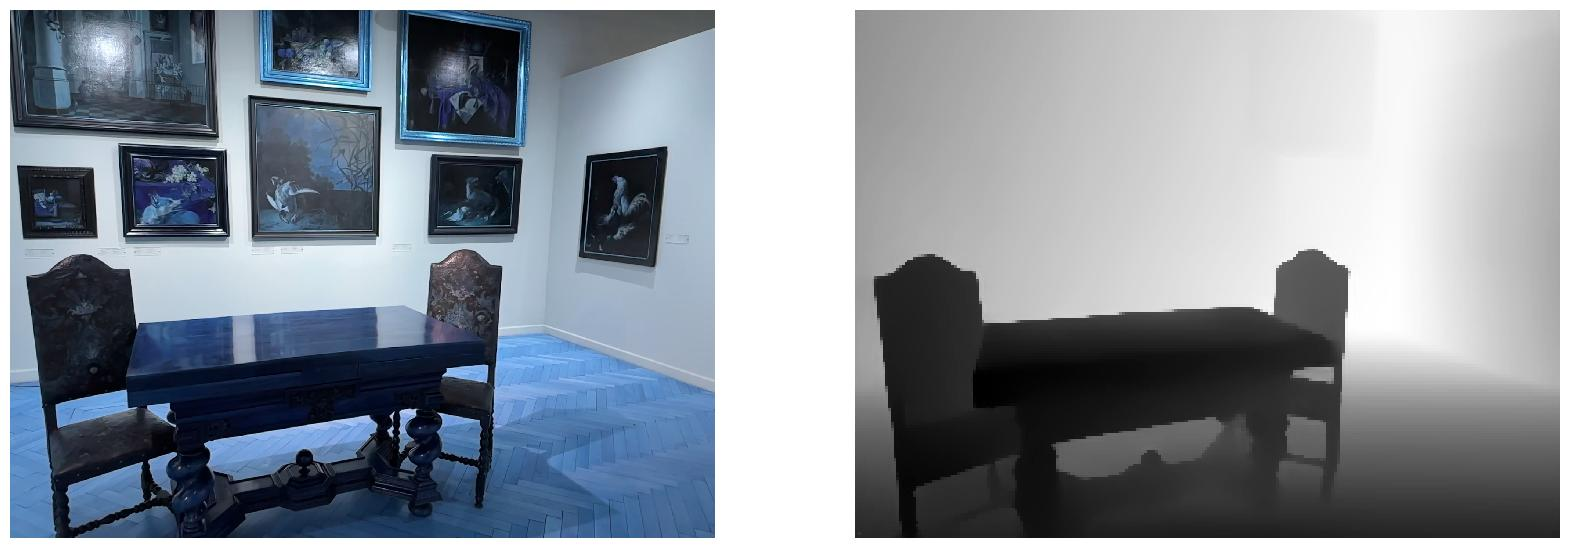
\includegraphics[width=0.9\textwidth]{dataset/plt_3e8e0ed8f8.jpg}
    \end{figure}
    \begin{figure}[H]
        \centering
        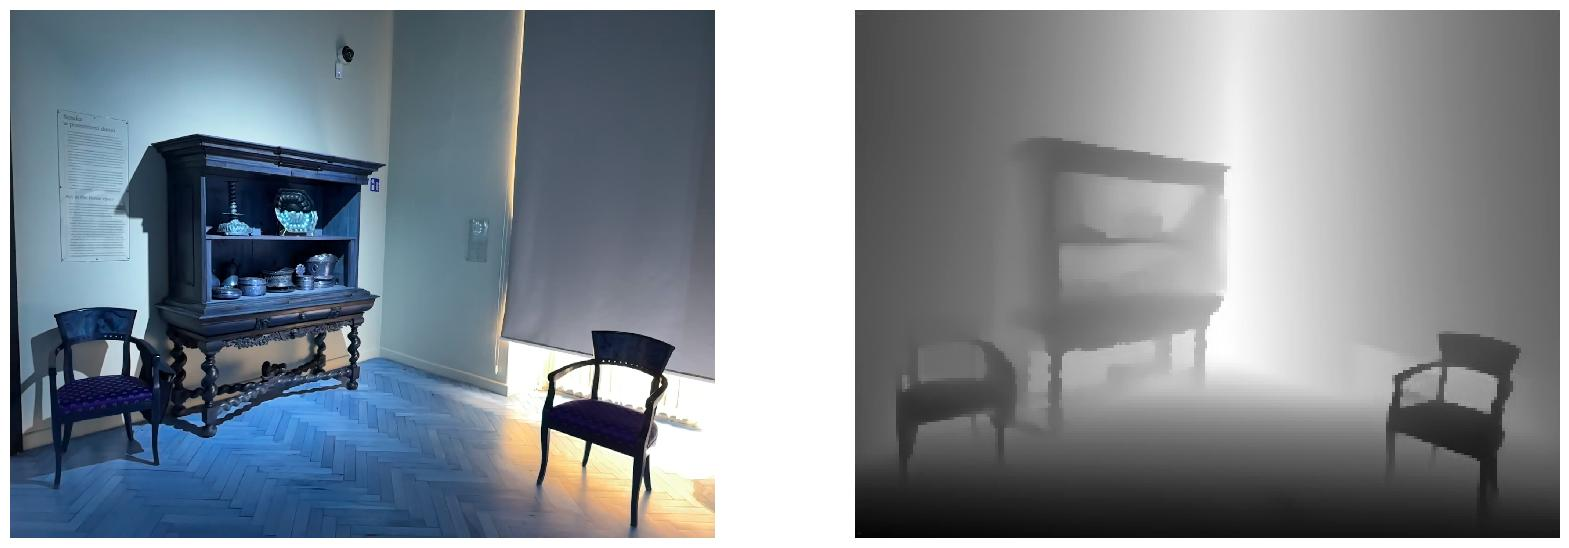
\includegraphics[width=0.9\textwidth]{dataset/plt_b317492e59.jpg}
    \end{figure}
    \begin{figure}[H]
        \centering
        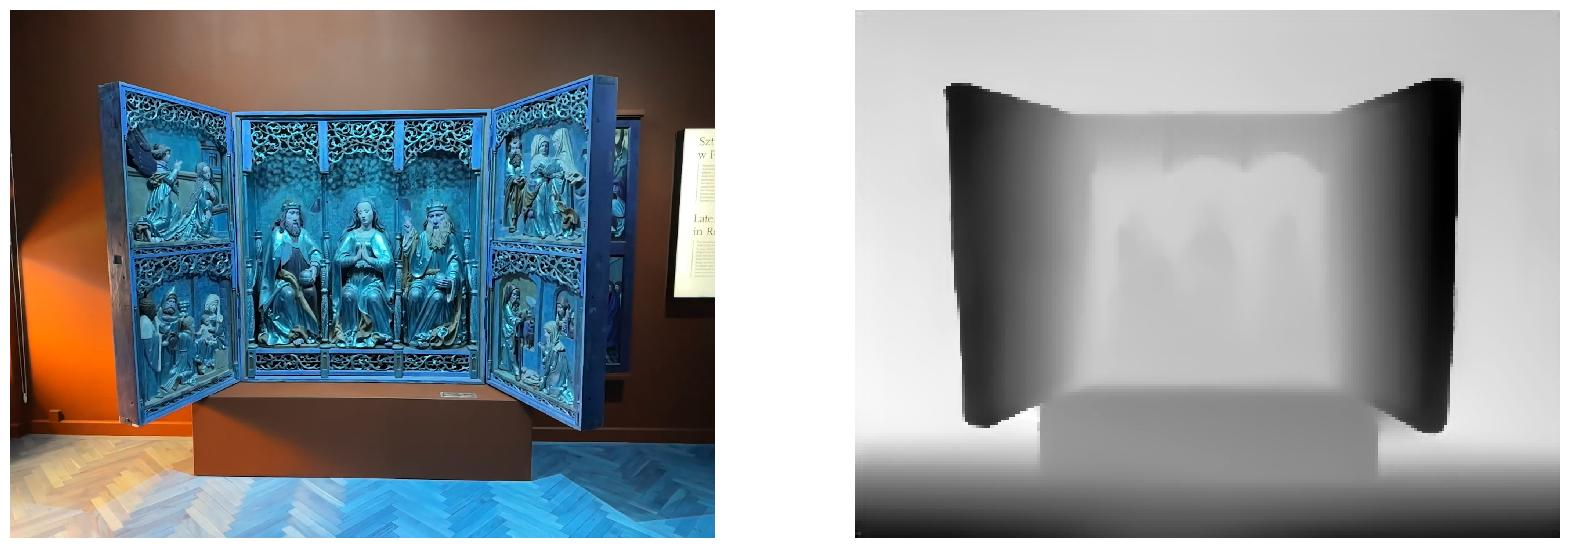
\includegraphics[width=0.9\textwidth]{dataset/plt_4ca5add536.jpg}
    \end{figure}
    \begin{figure}[H]
        \centering
        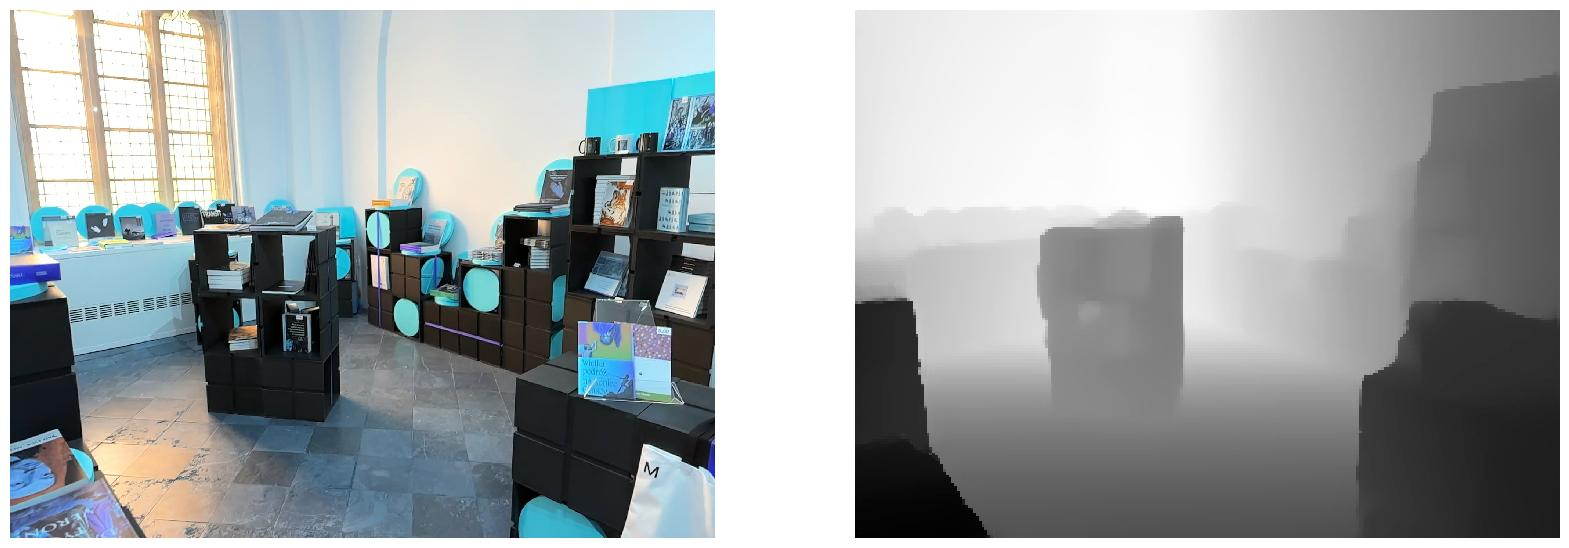
\includegraphics[width=0.9\textwidth]{dataset/plt_c5d7b9b753.jpg}
    \end{figure}
    \begin{figure}[H]
        \centering
        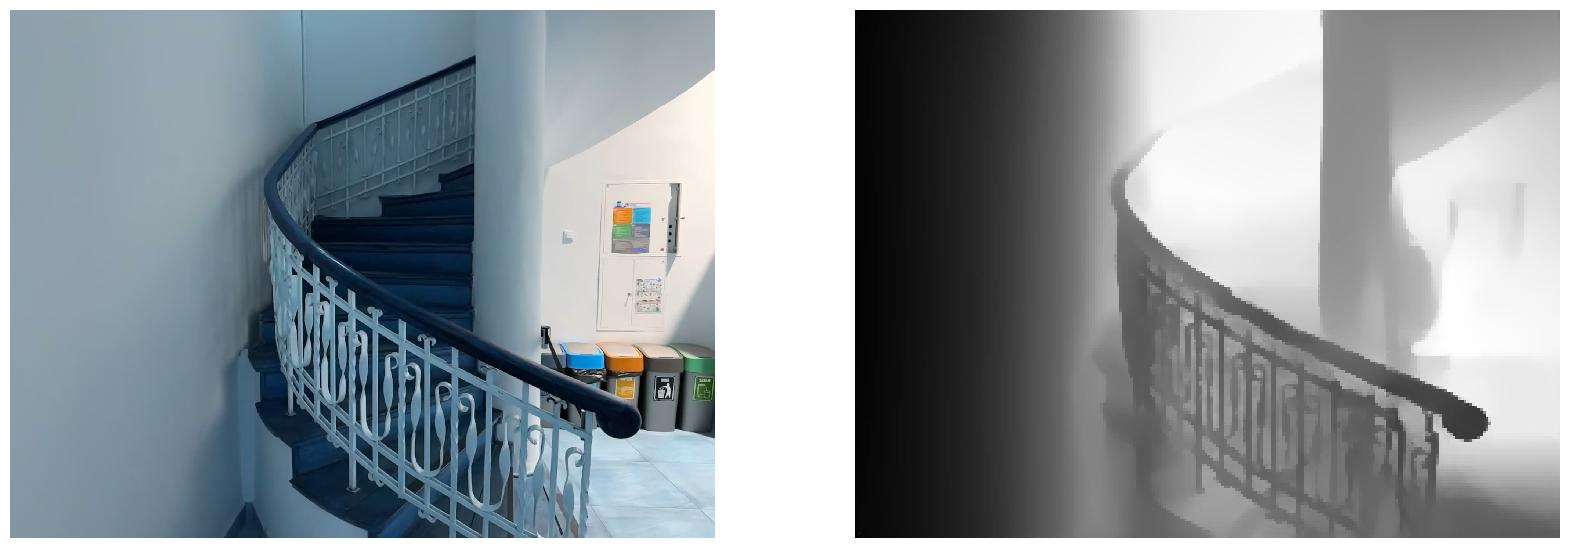
\includegraphics[width=0.9\textwidth]{dataset/plt_4e4a7402d2.jpg}
    \end{figure}
    \begin{figure}[H]
        \centering
        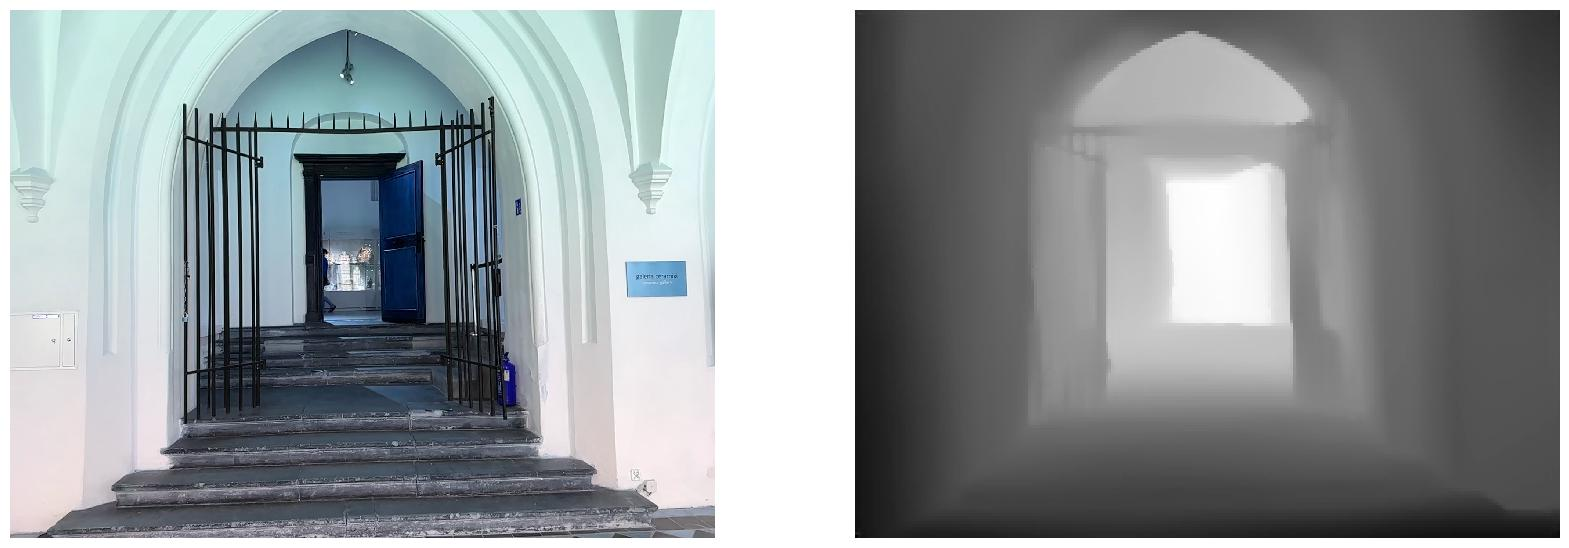
\includegraphics[width=0.9\textwidth]{dataset/plt_5e9e52fd8e.jpg}
    \end{figure}
    \begin{figure}[H]
        \centering
        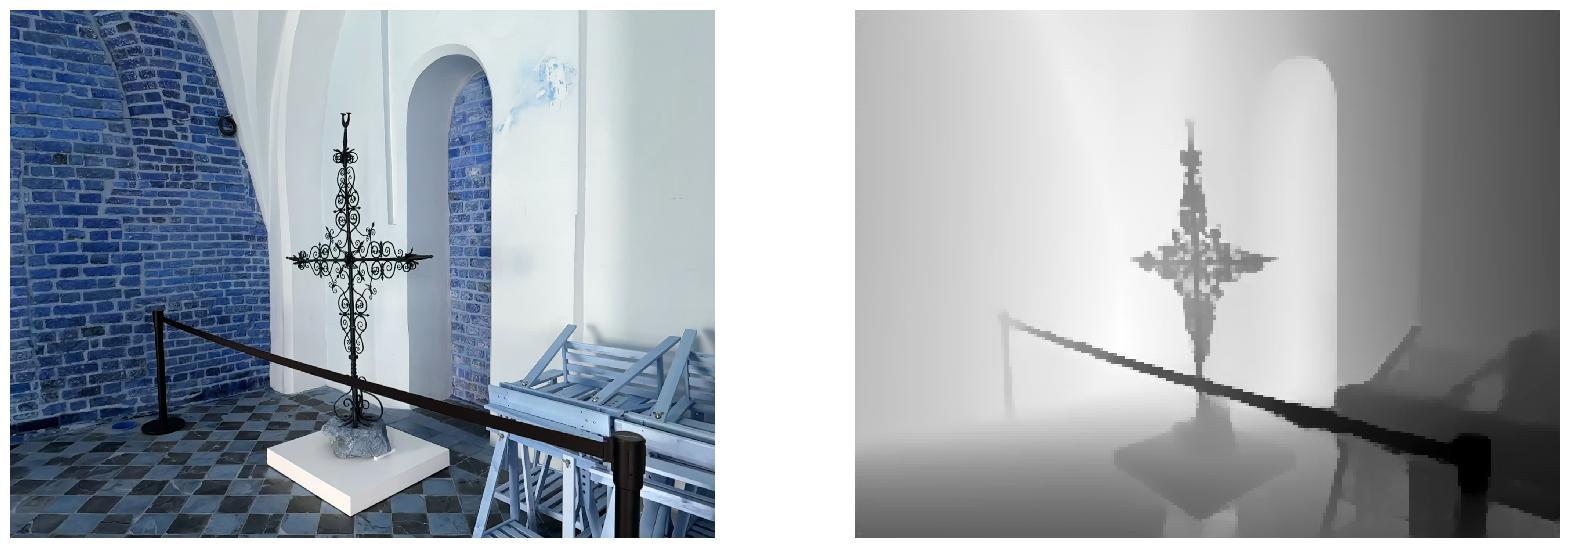
\includegraphics[width=0.9\textwidth]{dataset/plt_6fc547c962.jpg}
    \end{figure}
    \begin{figure}[H]
        \centering
        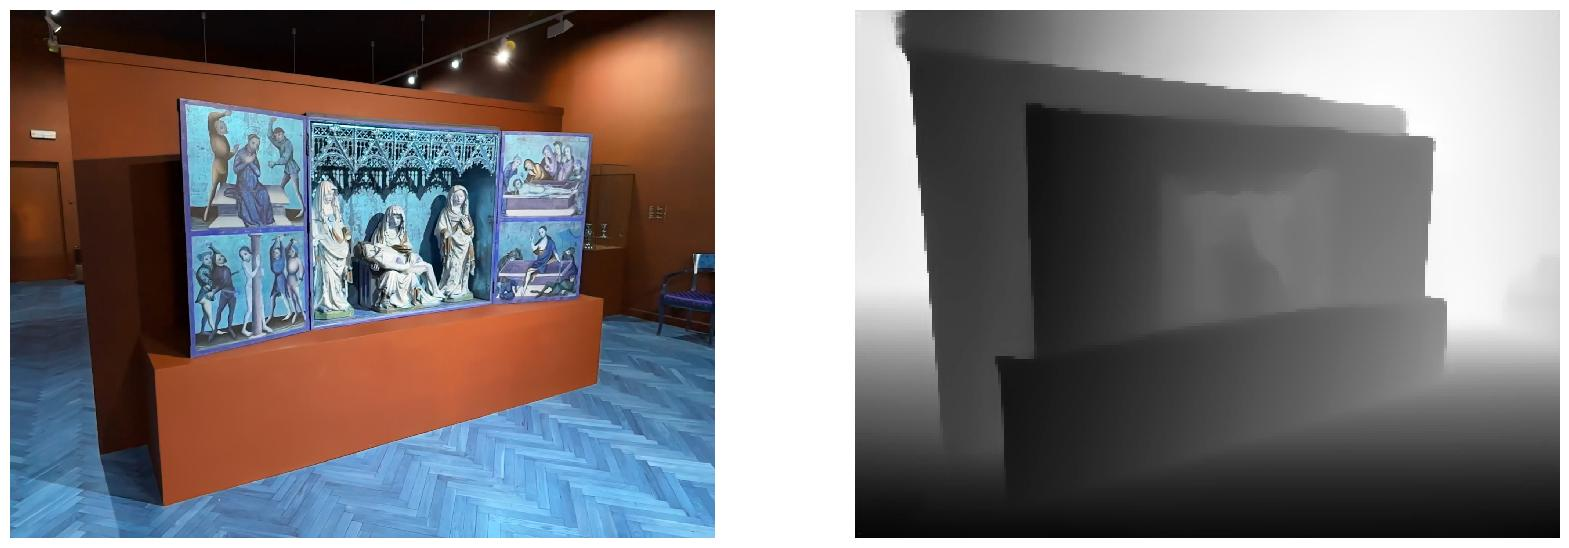
\includegraphics[width=0.9\textwidth]{dataset/plt_53e9714fcc.jpg}
    \end{figure}
    \begin{figure}[H]
        \centering
        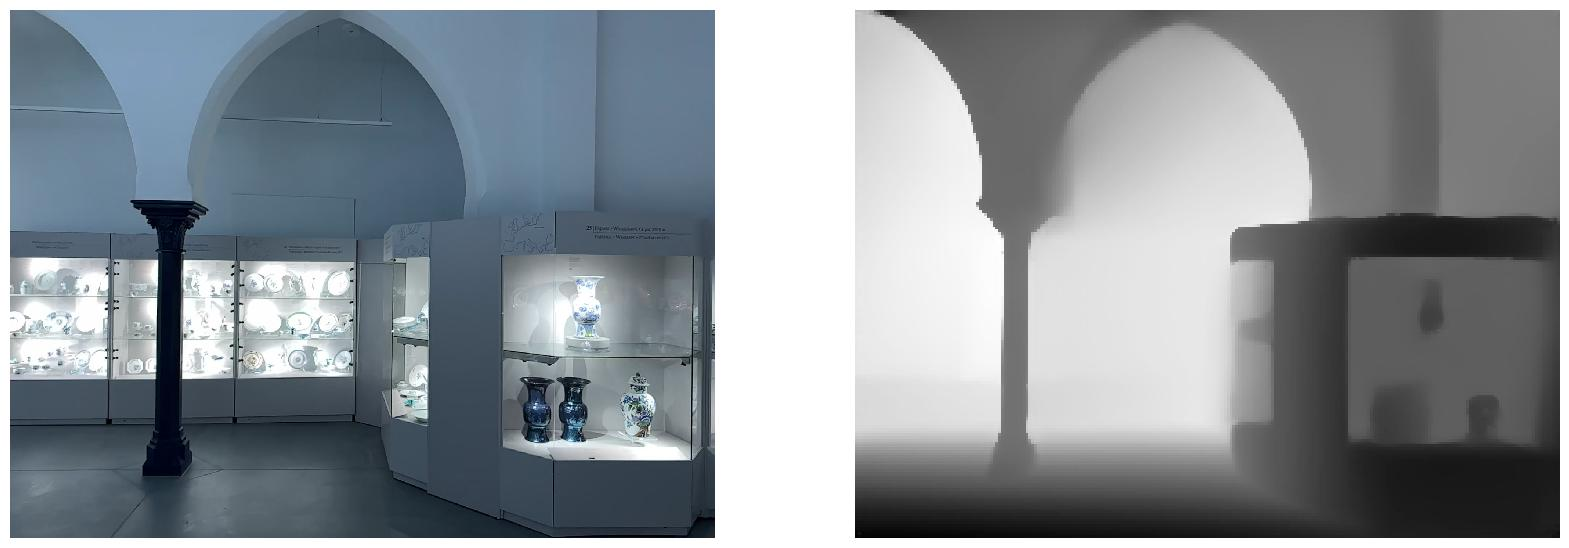
\includegraphics[width=0.9\textwidth]{dataset/plt_80eb280b51.jpg}
    \end{figure}
    \begin{figure}[H]
        \centering
        \includegraphics[width=0.9\textwidth]{dataset/plt_a451468719.jpg}
    \end{figure}
    \begin{figure}[H]
        \centering
        \includegraphics[width=0.9\textwidth]{dataset/plt_af49f6f8f8.jpg}
    \end{figure}
    \begin{figure}[H]
        \centering
        \includegraphics[width=0.9\textwidth]{dataset/plt_c757c940d1.jpg}
    \end{figure}
    \begin{figure}[H]
        \centering
        \includegraphics[width=0.9\textwidth]{dataset/plt_cc90b4fd22.jpg}
    \end{figure}
    \begin{figure}[H]
        \centering
        \includegraphics[width=0.9\textwidth]{dataset/plt_dda4834a30.jpg}
    \end{figure}

    \begin{figure}[H]
        \centering
        \includegraphics[width=0.9\textwidth]{dataset/plt_69c7b295e8.jpg}
    \end{figure}
    \begin{figure}[H]
        \centering
        \includegraphics[width=0.9\textwidth]{dataset/plt_ed7155d95c.jpg}
    \end{figure}
    \begin{figure}[H]
        \centering
        \includegraphics[width=0.9\textwidth]{dataset/plt_b7aa15fa2e.jpg}
    \end{figure}
    \begin{figure}[H]
        \centering
        \includegraphics[width=0.9\textwidth]{dataset/plt_a1179cc06a.jpg}
    \end{figure}
    \begin{figure}[H]
        \centering
        \includegraphics[width=0.9\textwidth]{dataset/plt_2331b84e7d.jpg}
    \end{figure}
    \begin{figure}[H]
        \centering
        \includegraphics[width=0.9\textwidth]{dataset/plt_2351129738.jpg}
    \end{figure}
    \begin{figure}[H]
        \centering
        \includegraphics[width=0.9\textwidth]{dataset/plt_e699030ce9.jpg}
    \end{figure}
    \begin{figure}[H]
        \centering
        \includegraphics[width=0.9\textwidth]{dataset/plt_0cacd83d9e.jpg}
    \end{figure}
    \begin{figure}[H]
        \centering
        \includegraphics[width=0.9\textwidth]{dataset/plt_c5830d92d4.jpg}
    \end{figure}
    \begin{figure}[H]
        \centering
        \includegraphics[width=0.9\textwidth]{dataset/plt_730fe44f49.jpg}
    \end{figure}
    \begin{figure}[H]
        \centering
        \includegraphics[width=0.9\textwidth]{dataset/plt_91cfb2b50f.jpg}
    \end{figure}
    \begin{figure}[H]
        \centering
        \includegraphics[width=0.9\textwidth]{dataset/plt_77a926f35d.jpg}
    \end{figure}
    \begin{figure}[H]
        \centering
        \includegraphics[width=0.9\textwidth]{dataset/plt_02b48acb11.jpg}
    \end{figure}
    \begin{figure}[H]
        \centering
        \includegraphics[width=0.9\textwidth]{dataset/plt_c87d38b94d.jpg}
    \end{figure}
    \begin{figure}[H]
        \centering
        \includegraphics[width=0.9\textwidth]{dataset/plt_0a8dd7d7bc.jpg}
    \end{figure}
    \begin{figure}[H]
        \centering
        \includegraphics[width=0.9\textwidth]{dataset/plt_dd711377c4.jpg}
    \end{figure}
    \begin{figure}[H]
        \centering
        \includegraphics[width=0.9\textwidth]{dataset/plt_d4be149153.jpg}
    \end{figure}
    \begin{figure}[H]
        \centering
        \includegraphics[width=0.9\textwidth]{dataset/plt_c982ac237d.jpg}
    \end{figure}
    \begin{figure}[H]
        \centering
        \includegraphics[width=0.9\textwidth]{dataset/plt_03a2c730c8.jpg}
    \end{figure}

\end{easyappendix}